The underlying mechanism which causes timing noise is not understood. Since the
first discussions in \citet{Boynton1972} multiple models have been proposed
which are able to describe some of the features. However, the variety of ways
timing noise manifests and the uncertainty in the mechanisms at work have made
it difficult for any conclusive statements to be made about the models. A
complete understanding of timing noise must not only explain the observed
variations, but also remain consistent with our understanding of neutron stars
derived from other observations such as glitches. A complicating factor in
understanding timing noise is that the observed features have timescales
similar to the duration that we have been able to observe pulsars; it is
therefore possible, as noted by \citet{Hobbs2010}, that observations which look
like a random walk over a short timescale, may in fact be periodic or something
else entirely over longer timescales.  Observations of new features prompt new
models for timing noise; as a result the timing noise interpretations have
evolved with the observations. In this section, we will present an overview of
these interpretations and the existing evidence which supports them.

\subsection{Random walk models}
\label{sec: TN interpretations random walk models}

Timing noise was first quantified and interpreted by \citet{Boynton1972} as a
Poisson like random walk in one of the phase, frequency, or spin-down. The
pulsar spins down according to the power law spin-down of Eqn.~\eqref{eqn:
power law spin-down} except that at random times the pulse phase, frequency, or
spin-down will undergo a sudden discontinuity. The waiting times between such events
are Poisson distributed with a rate $\lambda$ such that over a period $T$ the number of
events follows a Poisson distribution with mean $\lambda T$. All the jumps are
independent and the magnitudes are randomly distributed with means given by
$\langle\Delta\phi\rangle$, $\langle\Delta\nu\rangle$, and $\langle\Delta\dot{\nu}\rangle$ for the phase,
frequency, and spin-down.

\citet{Boynton1972} and others since investigate the statistical properties of
such random walks by splitting the phase evolution into contributions from the
secular spin-down $\phi_{\mathrm{S}}$, as given by Eqn.~\eqref{eqn: Taylor
compact}, and contributions from the random walks $\Delta\phi_\mathrm{R}$ such
that the total phase evolution is given by
\begin{equation}
    \phi = \phi_{\mathrm{S}} + \Delta\phi_{\mathrm{R}}.
\end{equation}
The three random walks can be written as the sum of $N$ individual events
occurring at times $t_{i}$
\begin{align}
    \Delta\phi_{\mathrm{R}} & = \s{i=1}{N}\Delta\phi_{i} H(t - t_{i})
     && \mathrm{(phase),} \\
    \Delta\phi_{\mathrm{R}} & = \s{i=1}{N}\Delta\nu_{i} (t-t_{i})H(t - t_{i})
     && \mathrm{(frequency),} \\
    \Delta\phi_{\mathrm{R}} & = \s{i=1}{N}\frac{1}{2}\Delta\dot{\nu}_{i} (t-t_{i})^{2}H(t - t_{i})
     && \textrm{(spin-down),}
\end{align}
where $H(t)$ is the Heaviside step function. It should be noted that in this
treatment the three types of noise are considered separately such that timing
noise residuals from either a random walk in phase, frequency, or spin-down;
work by \citet{Cordes1980} extended this model to handle mixing between the
types of noise.

The timing residuals can be calculated by fitting and removing a second order
Taylor expansion, provided the perturbations
of $\phi_{\mathrm{s}}$ are small then the remainder will be exactly given by
$\phi_{\mathrm{s}}$. Then, as described by \citet{Boynton1972}, we can
average over the $\Delta\phi_{i}, \Delta\nu_{i}$, or $\Delta\dot{\nu}_{i}$
distributions, the $t_{i}$ distribution, and the $N$ distributions to give
\begin{align}
    \langle \Delta\phi_{R} \rangle & = \langle \Delta\phi \rangle \lambda T
    %= S_{\mathrm{PN}}T 
    && \mathrm{(phase),} \\
    \langle \Delta\phi_{R} \rangle & = \frac{1}{2}\langle \Delta\nu \rangle \lambda T^{2}
    %= \frac{1}{2}S_{\mathrm{FN}}T^{2} 
    && \mathrm{(frequency),} \\
    \langle \Delta\phi_{R} \rangle & = \frac{1}{6}\langle \Delta\dot{\nu} \rangle \lambda T^{3}
    %= \frac{1}{6}S_{\mathrm{SN}}T^{3} 
    && \textrm{(spin-down).}
\label{eqn: RW comps}
\end{align}
%Here we have implicitly defined the strength parameters which combine the rate
%and averaged magnitude of jumps into a single quantity. Measurements of timing
%noise, if they are discreet events, will observe the accumulation of many
%individual events. As a result only the strength can be
%measured, not the rate and average magnitude.

The three types of noise are distinguishable by their dependence on the
observation time $T$. The type of noise can be measured by translating this
into the standard deviation of $\Delta\ddot{\nu}$ after fitting a cubic polynomial.
Using this method, \citet{Boynton1972} categorised timing noise in
the Crab pulsar as `frequency-like' noise.  They found that over a $5$~year
period the noise process was stationary and consistent with the frequency noise
hypothesis. No deterministic process could account for the timing residuals
strengthening their conviction that some random process was taking place.
However, they suggested that over longer periods the random walk will be
non-stationary due to mixing with other types of walks.

The interpretation of timing noise as a Poisson random walk is a purely
empirical statistical model. It is however backed up for a rich variety of
possible substantive physical models.  A key feature of any physical random
walk model is that it must be able to produce both increases and decreases in
the relevant parameter. For this reason, it is felt unlikely that the mechanism
responsible for a random walk timing noise model is the same as model proposed
to explain glitches. Since it is assumed that the number of events
is large so that we can take a statistical average, this does not test if the
process is indeed discreet, or if it is continuous.

The first substantive physical model to explain the random walk was proposed by
\citet{Boynton1972}, the noise process consisted of the accretion of small
lumps of matter onto the NS from the interstellar medium. Lumps of matter fall
randomly onto the surface of the star causing either a spin-up or spin-down
through the transfer of angular momentum. After this, many models were proposed
such as small starquakes and the random pinning and unpinning of vortex lines; these
were reviewed by \citet{Cordes1981} and evaluated against observational
constraints. Of these, only three mechanisms where found to be consistent with
observations: crust breaking by vortex pinning, a response to heat pulses, and
luminosity related torque fluctuations. Since this review, new random walk
mechanisms have been proposed such as: variations in the magnetospheric gap
size \citep{Cheng1987}; the interference by debris entering the magnetosphere
\citep{Cordes2008}; and the accumulation of multiple micro-glitches
\citep{Janssen2006}. It would be a useful exercise to review both the new and
old mechanisms against the current observational catalogue since new and
improved observations may better constrain some of these physical models.

The first measurement of individual events was made by \citet{Cordes1985} who
identified $\sim20$ events in both frequency and spin-down which could not be
explained by a glitch. In the same work, considering 24 pulsars over a period
of~$\sim13$~years, the authors concluded that: the timing noise seen in the
data could not be explained solely by an idealised random walk processes in the
phase, or its derivatives. They suggested that most of the activity is due to a
mixture of events in the phase, frequency and/or frequency derivative.

A recent observational review of timing noise was performed by
\citet{Hobbs2010} for 366 pulsars, the authors do not comment on whether these
observations constrain random walk models. Instead, they conclude that, when
observed on sufficiently long time scales, the residuals which may before have
looked like a random walk, contained quasi-periodic features. It is impossible
to argue that this is not the case for pulsars which only display random-walk
features over current observation periods, since the quasi-periodicity may have
periods longer than the observation. This effect is apparent for the Crab
pulsar which was found by \citet{Boynton1972} to be consistent with
frequency-like noise, but in Fig.~\ref{fig: timing noise example} we
see quasiperiodic features. In conclusion, in agreement with \citet{Hobbs2010}
we find that a pure random walk hypothesis is not entirely consistent with
observations. However, if one simply wants to characterise timing-noise over
short periods of data, a random walk provides a good emperical description.

\subsection{Free precession}
\label{sec: free precession}

A mechanism which could quite naturally produce strictly periodic variations in
the observable features of a pulsar is \emph{free precession}. This occurs in
any non-spherical rigid body for which the angular momentum is not aligned with a
principle axis of the moment of inertia. Such a circumstance could arise given
the chaotic birth of NSs. However, we must be clear that the timing noise
induced by precession alone would be strictly deterministic; this is something
which we do not typically observe except in a handful of pulsars, one of which
is considered in Chapter.~\ref{sec: testing models}. We will now
consider the mechanics of free precession.

In the simplest case, we take a biaxial body,
rotating about an axis $\Omega$, with a moment of inertia given by
\begin{equation}
    I = \left[\begin{array}{ccc}
            I_{0} & 0 & 0 \\
            0 & I_{0} & 0 \\
            0 & 0 & I_{0} + \Delta I
            \end{array}\right],
\end{equation}
where $I_0$ is the total moment of inertia of the star involved in precession
and $\Delta I/I_0$ is the measure of oblateness or prolateness. If the
body is free from torques, then in the rotating frame of the body, Euler's
equations of motion \citep{Landau1969} are given by
\begin{equation}
    I\dot{\bm{\Omega}} + \bm{\Omega} \times \left(I\bm{\Omega}\right)=0.
\end{equation}
This is a system of three coupled ODEs. Writing the components of the spin
vector as $\bm{\Omega} = [\Omega_{x}, \Omega_{y}, \Omega{z}]$ and
defining $\epsI = \Delta I / I_0$, we have the
set of equations:
\begin{align}
\dot{\Omega}_x = -\epsI \Omega_y\Omega_z, &&
\dot{\Omega}_y = \epsI \Omega_x \Omega_z, &&
\dot{\Omega}_z = 0
\end{align}
We can find a solution by first setting $\Omega_{z}=\mathrm{const}$.
We are then left with a set of
two coupled ODEs, solving these with appropriate initial conditions
the solutions take the form
\begin{align}
\begin{split}
    \Omega_{x} & = \Omega_{0}\sin(a_0)\sin\left(\Omega_{0}\cos(a_0)\epsilon t\right), \\
    \Omega_{y} & = \Omega_{0}\sin(a_0)\cos\left(\Omega_{0}\cos(a_0)\epsilon t\right),\\
    \Omega_{z} & = \Omega_0 \cos(a_0),
\label{eqn: free precession}
\end{split}
\end{align}
where $a_0$ is the angle between the spin-vector and the body frame $z$ axis, and
$\Omega_0$ is the magnitude of the spin-vector.

We observe that the spin axis of the body will trace out a cone about the $z$
principle axis of the moment of inertia with a period of
\begin{align}
\tau_P = \frac{1}{\Omega_{z}\epsilon}.
\label{eqn: tauP free}
\end{align}
The half-angle of the cone is set by the
initial conditions and will not evolve. This is the motion of free precession
and is illustrated in Fig.~\ref{fig: precession}.
\begin{figure}[htb]
\centering
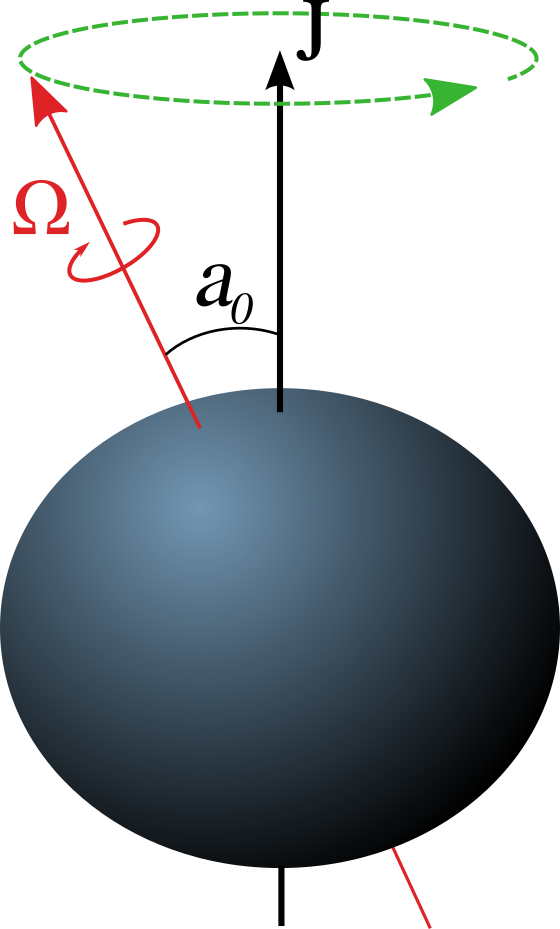
\includegraphics[scale=0.2]{Precession.png}
\caption{Illustration of free precession for a simple biaxial body. The spin
    axis $\mathbf{\Omega}$ traces out a cone about the angular momentum vector $\mathbf{J}$.}
\label{fig: precession}
\end{figure}•

Neutron stars are assumed to have a solid crust, as such they may be
non-axially symmetric. Precession, as a candidate to explain timing noise
fluctuations, was first discussed by \citet{Ruderman1970}. He found that the
free precession period was, for reasonable values of the  ellipticity
$\epsilon$, able to explain periodic fluctuations in the Crab pulsar.
Precession is one of the few periodic mechanism that could act on neutron star
with the typical periods observed in typical timing residuals.

However, the superfluid unpinning interpretation for glitches poses a problem for
sustained free precession as an interpretation of timing noise. If correct,
then the interior of a neutron star must contain a superfluid component pinned
to the crust. It was shown by \citet{Shaham1977} that for perfect pinning the
deformation of the star is modified resulting in
\begin{align}
\epsilon = \frac{\Delta I}{I_0} + \frac{I_{\textrm{psf}}}{I_0},
\end{align}
where $I_\textrm{psf}$ is the moment of inertia of the superfluid pinned to the
crust. To explain the magnitude of observed glitches this second term was found
to be $\sim 0.01$. Inserting this into Eqn.~\eqref{eqn: tauP free}, we see that
the free precession period must be approximately 100 times the spin-period. Therefore,
the existence of a perfectly pinned superfluid precludes long-period precession
where the precession period is millions of times longer than the spin-period.

Despite the inconsistency with the superfluid pinning model for glitches,
evidence was presented by \citet{Stairs2000} of free precession in pulsar
B1828-11. They found the phase residuals and variations in the pulse profile
could be accounted for by precession. This pulsar has been studied by others
since and in Chapter.~\ref{sec: testing models} we will discuss this pulsar and
the precession interpretation in more detail.

One resolution to this comes from relaxing the assumption that the superfluid
pinning is perfect. \citet{Sedrakian1999} found that imperfect pinning of the
superfluid allows long-lived precession with damping. It is therefore possible,
as noted by \citet{Cordes1993} that free precession may be excited by torque
fluctuations that counter the damping process; in turn, the precession can
drive torque fluctuations. However, there remains some uncertainty as to the
details of this model so whether precession can coexist with a superfluid core
remains an open question. Resolving this, and determining exactly how the
models are incompatible is an important task which we hope to make some headway
on in this thesis by studying the case for precession in Chapter.~\ref{sec:
testing models}.


\subsection{Magnetospheric switching}
\label{sec: two state switching}

Recently a new model has been proposed by \citet{Lyne2010} to explain the
observation that of quasi-periodicity in timing noise structure.
This work was motivated by the observations of \citet{Kramer2006} that the
pulses from PSR~B1931+24 where intermittent: the pulsar acts as a normal pulsar
for $\sim10$~days and then switches off, being undetectable for $\sim25$~days,
before switching on again. This behaviour can be understood as the pulsar switching
between two states. Analysing the spin-down rate between the on and off
states, they determined the spin-down rate $\dot{\nu}$ was $\sim50\%$ faster in
the on state. The figure illustrating this is reproduced in Fig.~\ref{fig:
kramer 2006 fig2}.
\begin{figure}
    \centering
    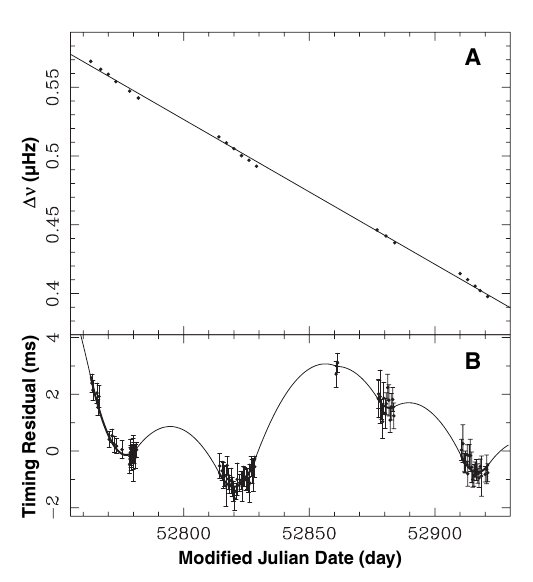
\includegraphics[width=.5\textwidth]{Kramer_2006_fig2}
    \caption{Figure taken from \citet{Kramer2006} showing the switched spin-down
             of pulsar PSR B1931+24}
    \label{fig: kramer 2006 fig2}
\end{figure}
The  upper panel, Fig.~\ref{fig: kramer 2006 fig2}\textbf{A}, shows the
evolution of the rotational frequency over a 160 day period encompassing
several switching events. The line shows the long-term averaged spin-down of
the pulsar while the dots show individual measurements made during the on
state. During these on states, the gradient of the reduction in frequency is
increased: the spin-down rate is faster.  It is thought that measurements of
the frequency in the off state would produce a line with decreased spin-down
connecting the dots. Plotted in Fig.~\ref{fig: kramer 2006 fig2}\textrm{B} is
the timing residual; this shows significant quasi-periodic modulations
correlated with the switching.

PSR~B1931+24 evidently switches suddenly and periodically between two distinct
states. The authors, \citet{Kramer2006}, realised that the neutron star
magnetosphere is the only mechanism which could produce such sharp changes with
correlated changes in the spin-down rate and beam.  It intuitively makes sense
that magnetospheric state which does not produce EM emission may have a lower
spin-down rate while the state which does produce radiation has a higher
spin-down rate.

Motivated by this observation, the authors of \citet{Lyne2010} tested a range
of other pulsars and presented a study of 17 pulsars for which they found
evidence for `two-state magnetospheric switching'. Unlike in PSR~B1931+24,
these pulsars are not intermittent, but are seen to continuously pulse. The
authors measured changes in the spin-down rate $\dot{\nu}$ of each pulsar by
using what we will call in this thesis the \emph{observer-method}. This
consists of fitting a Taylor expansion to short segments of data of duration
$T$, in each segment the fitted coefficient $\dot{\nu}$ is taken as a
measurement of the spin-down rate at the mid-point of the segment. Repeating
this process in a sliding window at intervals $T/4$ throughout the whole data set gives the
evolution of the spin-down rate over the entire observation.  Over a
$\sim20$~year period they found a variety of smooth periodic fluctuations with
typical periods of years. In Fig.~\ref{fig: lyne 2010 fig2} we reproduce their
original plot showing the periodic variations in spin-down rates.
\begin{figure}
    \centering
    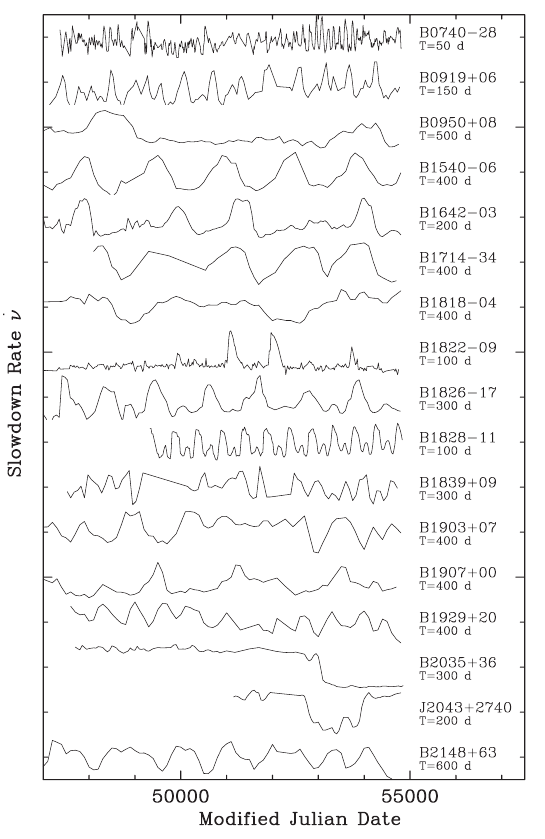
\includegraphics[width=.5\textwidth]{Lyne_2010_fig2}
    \caption{Figure adapated from \citet{Lyne2010} showing the spin-down rate
             of 17 pulsars over a $\sim20$~year period.}
    \label{fig: lyne 2010 fig2}
\end{figure}

The method used to calculate the spin-down in Fig.~\ref{fig: lyne 2010 fig2}
required time averaging; the baseline used $T$ is given below the pulsar name
on the right-hand side of the plot, typically $T\sim100$~days. The authors of
\citet{Lyne2010} argue that, if the pulsar is in fact switching between
magnetospheric states, then its spin-down rate will be periodically switching
between at least two values. In the event that the switching occurs over
timescale comparable to the time averaging baseline, the resulting time averaged
spin-down rate will be smoothed out. Therefore, the smooth periodic variations in
Fig.~\ref{fig: lyne 2010 fig2} could be produced by the spin-down rate
switching between two (or more) well defined values.

If the switching was magnetospheric in origin, then \citet{Lyne2010} realised
that changes in the spin-down rate should correlate with changes in the
beam-shape.  They found that for 6 pulsars the pulse width did indeed correlate
with changes in the spin-down rate, although for some pulsars this was an
anticorrelation rather than a correlation. However, like the spin-down rate
these pulse shape variations are also smooth and subject to the same time
averaging process. 

To test if the mechanism causing these variations is smooth or instantaneous
(i.e. switching) the authors needed to look at an observed property not subject
to the time-averaging process.  This is possible by looking at individual
measurements of the pulse width which are taken during each short $\sim30$~mins
observation. In this way, they are time averaged over a duration much shorter
than the modulation period and could, in principle, resolve individual
switching events. They were able to do this for two pulsars, B1822-09 and
B1828-11, and argue that the individual beam-width measurements, by eye, can be
interpreted as taking one of two values with few observations seen in between.
They took this as evidence that the pulsars were indeed undergoing sudden,
instantaneous, and periodic switching between two states. We note that the
stronger of these two condidates, B1828-11, was previously discussed in the
context of free precession in Sec.~\ref{sec: free precession}.

Since this initial study, evidence for switching in two others pulsars have
been reported by \citet{Perera2014} and \citet{Perera2016} with additions added
to the model in terms of the detail of the switching. However, so far the
magnetospheric switching hypothesis is missing an underlying physical model
which both causes the switching between states and provides the clock regulating
the period.

\citet{Lyne2010} argue that the fast state changes seem to rule out free
precession as the origin of oscillatory behaviour observed in timing residuals,
in particular for B1828-11.

\citet{Jones2012} argues that such dismissal of precession is premature since
the modulation period of the switching has yet to be explained.  Instead, the
author raises the idea that precession and magnetospheric switching are not
mutually exclusive, but precession may in fact cause the switching. Pulsars are
most probably born in a randomly distributed magnetospheric state, at least
some may therefore exist under a delicate balance between two states.
Precession may be capable of periodically varying the statistical probability
of existing in one state or the other, sharp changes would be caused by an
`avalanche effect' as the particle energies reach a threshold.  This provides
the timescale for switching along with the ability for the switching to be
quasi-periodic since the precession only biases the probability.

Another idea proposed by \citet{Cordes2013} interpreted two state
switching as evidence for a system in a state of `stochastic resonance'.  This
occurs in systems in which, under certain conditions, a weak periodic forcing
function is amplified by stochastic noise. To explain this phenomenon in
Appendix~\ref{app: stochastic} we present a toy model of stochastic resonance
for a particle in a well. The switching could therefore be the result of any
periodic modulation, such as precession, coupled to random fluctuations. This
would quite naturally explain the stability of states, the timescales over
which the occur, and the fact that it is observed in only some pulsars.

As already mentioned, determining the cause of periodic modulations has
important implications for neutron star physics. Later on in Chapter~\ref{sec:
testing models} we will investigate this issue, particuarly in the context of
PSR~B1828-11, using a quantiative model comparison. In the remainder of this
section we will build a model for magnetospheric switching incorparating all
the ideas of \citet{Lyne2010} and \citet{Perera2014}; this model forms the basis
of the model compared against precession in Chapter~\ref{sec: testing models}.
Finally, in Sec.\ref{sec: switching predictions} we show how this simple
emperical model of switching makes a testable prediction which could be
checked by pulsar astronomers using current data.

\subsubsection{Simple empirical model}

In the supplementary material to \citet{Lyne2010}, the authors presented
results from a simple empirical switching model to demonstrate the resulting
phase residuals. In this section, we will similarly develop a simple model and
show the effect of switching on the time-averaged spin-down rate and phase
residuals.

We model a pulsar as spinning down in the usual way, except that its
magnetosphere periodically and suddenly switches between two different states which
we label $A$ and $B$. The star spends a time $t_A$ and $t_B$ in each state such
that $t_A+t_B$ gives the total period of switching. We then associate spin-down
rates, $\dot{\nu}_{A}$ and $\dot{\nu}_{B}$ to each of the states such that the
underlying spin-down rate is a square wave oscillating between these values.
Since we do not concern ourself in this description with the exact periods,
only the gross features, let us define the ratio of time spent state in state
$A$ and $B$ as $R = t_{B}/t_{A}$.

This is a purely deterministic model and, having generated the spin-down
values, we can integrate twice to get the phase. From the phase, we can use the
observer-method to calculate the time-averaged spin-down rate
$\langle\dot{\nu}\rangle$, or we can fit a polynomial to the entire phase
evolution and remove it to get a phase residual. This integration to the phase
and then applying the observer-method models the data collection mechanism so
that our resulting spin-down rate predictions are smooth.

In Fig.~\ref{fig: lyne example D=0} we show the underlying spin-down rate $\dot{\nu}$,
the time-averaged $\langle\dot{\nu}\rangle$, and phase residual (in cycles) for
some typical values. For the time-averaged spin-down rate we carefully chose
an averaging time similar to the switching period. For the final phase residual
we fit and remove a Taylor expansion up to $\ddot{\nu}$ and divide the residual
difference by the period in order to get the phase residual in cycles.
\begin{figure}[htb]
    \centering
    \includegraphics[]{{R_2.0_D_0}.pdf}
    \caption{A deterministic realisation of the Lyne switched spin-down model. The
             resulting structure in the time-averaged spin-down rate and the phase
             residuals are strictly periodic. This shows
             the underlying spin-down rate in the top panel, the time-averaged spin-down
             rate (calculated using the observer-method) in the second panel, and the phase residual in the bottom panel.}
    \label{fig: lyne example D=0}
\end{figure}

The phase residuals in Fig.~\ref{fig: lyne example D=0} are strictly periodic
which is inconsistent with the observed variations in the majority of pulsars
\citep{Hobbs2010}. To develop this, \citet{Lyne2010} added a probabilistic
'dither' $D$ in the waiting time between switches. Now we have periods
$t_{A}^{i}$ and $t_{B}^{i}$ which are Gaussian distributed with a mean of
$t_{A}$ and $t_{B}$ and a standard deviation $D t_{A}$ and $D t_{B}$. In
Fig.~\ref{fig: lyne example D=0.3} we repeat the results of Fig.~\ref{fig: lyne
example D=0} with $D=0.3$.
\begin{figure}[htb]
    \centering
    \includegraphics[]{{R_2.0_D_0.3}.pdf}
    \caption{A realisation of the Lyne model with a random element producing the
             observed quasi-period structure. For a description
    of the three panels see Fig.~\ref{fig: lyne example D=0}}
    \label{fig: lyne example D=0.3}
\end{figure}
This dither can be used to understand why the residuals and averaged spin-down
rate are quasi-periodic rather than strictly periodic. However, this model
is missing a substantive physical explanation, namely what causes the switching
and why it is quasiperiodic.

\subsubsection{Simple empirical model: four time periods} 

The time averaged spin-down rates in Fig.~\ref{fig: lyne example D=0} and
Fig.~\ref{fig: lyne example D=0.3} result from having two spin-down rates and
two durations which the system spends in those states. These results can be
contrasted with the spin-down rates of B1828-11 seen in Fig.~\ref{fig: lyne
2010 fig2}.  With only the ingredients described by \citet{Lyne2010}, it is not
possible to consistently replicate the double peaked spin-down rate variations
seen for this pulsar. A similar problem was faced by \citet{Perera2014} for
PSR~B0919+06, in response the authors devised the following solution. Rather
than introduce a third spin-down state, they simply required that the system
has four periods instead of two as in the original \citet{Lyne2010}
description; that is, we have four times $\tI{A}, \tI{B}, \tI{C},$ and $\tI{D}$
which sum up to the total period.
The system then switches between the two states four times during
a single cycle.  To illustrate this, in Fig.~\ref{fig: test lyne underlying} we
show a single cycle in which the four periods are $100$, $100$, $50$, and $100$
days.
\begin{figure}[htb]
    \centering
    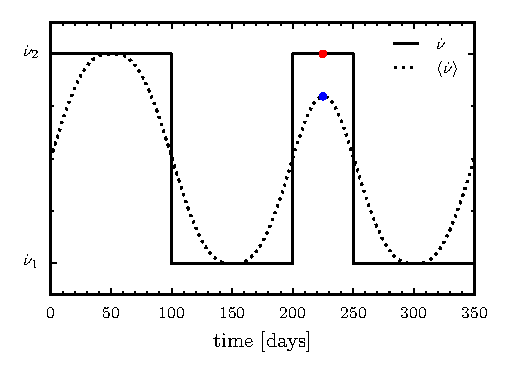
\includegraphics[]{TestLyneUnderlying}
    \caption{The spin-down rate $\dot{\nu}$ and its time-average $\langle\dot{\nu}\rangle$
    for a single cycle of the \citet{Perera2014} switching model in which the
    system switches between the two states four times during a single cycle.
    For the time-averaged spin-down rate, we have used a baseline of $100$~days,
    which is longer than the shortest period of $\tI{C}=$50~days; for this period we
    highlight the true spin-down rate by a red dot and the maximum time-average
    spin-down rate by a blue dot.}
    \label{fig: test lyne underlying}
\end{figure}

The \citet{Perera2014} switching model naturally produces the doubly peaked
time-averaged spin-down rate seen in B1828-11 when the time-averaging baseline is longer
than one of the switching periods. To explain more fully, when the time
averaging baseline is longer than a single period, then the time-average over
that section of the data will always include some amount of the other spin-down
rate. This can be seen in Fig.~\ref{fig: test lyne underlying} for the third
period which has duration 50~days, while the time averaging baseline is
100~days. In Fig.~\ref{fig: perera example}, we give the spin-down rate and
phase residual for this model to illustrate the variations in the residuals.
\begin{figure}[htb]
    \centering
    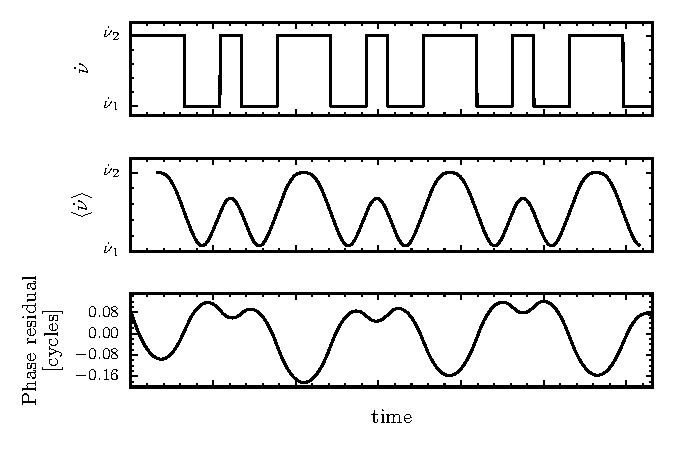
\includegraphics[]{Perera}
    \caption{Illustration of the \citet{Perera2014} extension to the
    \citet{Lyne2010} model in which the system switching between the two states
    four times per cycle, giving four independent switching periods. For a description
    of the three panels see Fig.~\ref{fig: lyne example D=0}}
    \label{fig: perera example}
\end{figure}

In Sec.~\ref{sec: switching} we will consider this switching
model further in the context of B1828-11 and develop a complete model for the
spin-down rate and beam-width modulations.

\subsubsection{A simple test of the switching hypothesis}
\label{sec: switching predictions}
PSR~B1828-11, which has a distinct doubly peaked spin-down, is one of two
pulsars for which the authors of \citet{Lyne2010} applied their magnetospheric
switching hypothosis too. Since
that result, several other pulsars have been found with a similar double-peaked
structure \citep{Perera2014, Perera2016}. In the previous section we introduced
a basic empirical model to explain this double-peak in the context of
magnetospheric switching. We will now describe a simple method to test this
switching hypothesis which so far, to our knowledge, has not been attempted,
but could be applied to current observational data.

If the double peaked spin-down rates of B1828-11, B0919+06, or any other pulsar
is due to the model proposed by \citet{Perera2014}, then the maximum spin-down rate
of the lower of the two peaks is a function of the time-averaging process and not
the pulsar itself.  Specifically, if the time-averaging was shorter than the
shortest period there would be no second lower peak: both peaks would have the same
value, $\dot{\nu}$.  Therefore, if one had access to the raw data used to
produce the time-averaged spin-down rate, one could repeat the time-averaging
process varying the time-averaging baseline which we denote by $T$. Then we
could imagine measuring the maximum spin-down rate of the two peaks in the
time-averaged spin-down rate and taking their ratio
\begin{align}
\mathcal{R} = \frac{\dot{\nu}_\textrm{max of lower peak}}
                   {\dot{\nu}_\textrm{max of larger peak}}.
\label{eqn: R-test}
\end{align}
Then, if the Perera switching model is to be believed, $\mathcal{R}$ should depend on $T$.

To demonstrate this, we can simulate the result numerically. We will do this by
varying the time averaging baseline for the simulation in Fig.~\ref{fig: test
lyne underlying} and calculating $\mathcal{R}$. The numerical results are
plotted in Fig.~\ref{fig: test lyne}.
\begin{figure}[htb]
    \centering
    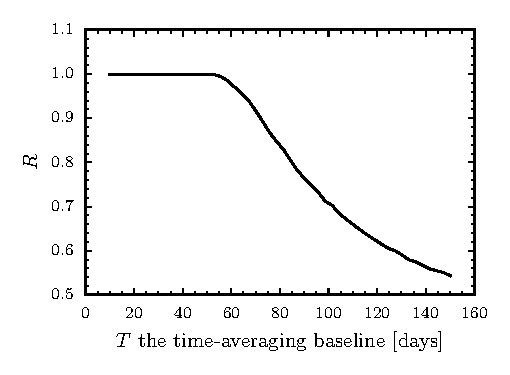
\includegraphics[]{TestLyne}
    \caption{Demonstration of the variations in $\mathcal{R}$, defined in
             Eqn.~\eqref{eqn: R-test}, in response to changing the time averaging
             baseline, $T$}
    \label{fig: test lyne}
\end{figure}
This clearly shows that for $T\le50$~days, when the time averaging baseline is
shorter than the shortest switching duration $\tI{C}$ (see Fig.~\ref{fig:
perera example}), $\mathcal{R}=1$ because the two peaks are of equal size.  For
$T>50$~days, $\mathcal{R}$ decreases until $T=150$~days, above this the
time-averaging is of a similar length to the total period of switching and so
we can't resolve any of the features.

We have shown that variations in the ratio of the two peaks in spin-down rate
would provide clear evidence in support of the \citet{Perera2014} model. Of
course in this example we have considered a simple situation where we have
known apriori which peak is being underestimated due to the observer-method of
calculating the time averaged spin-down rate. In real data, the situation may
be more complicated: it could be that it is the trough which is overestimated
instead of the peak being underestimated; or more than one switching duration
may be shorter than the time averaging baseline.  Nevertheless, the changing
ratio of the two peaks (or troughs) may still prove a simple way to test the
Perera model.

%\subsection{Evidence from anomalous braking indices}
%\label{sec: evidence from anomalous braking indices}
%
%An alternative motivation to study timing noise comes from the measurement of
%anomalous braking indices. The pulsar braking index is defined by $n$ in
%equation \ref{eqn: power law spin-down}.  Rearranging this equation as in
%\eqref{eqn: measured braking index} the braking index can be measured for
%observed pulsars. Different types of braking exhibit different braking indices.
%It is therefore a reasonable idea to measure the braking index and calculate
%the type of braking. Pulsars spun down by an electromagnetic torque should
%follow a braking index of $n=3$, while gravitational wave spin-down has $n=5$.
%
%Measuring these indices for the known pulsar population we do not find a consensus
%on the type of braking. Values from from unity up to $10^{6}$ and even negative
%braking indices have been measured. These are known as \emph{anomalous}
%braking indices.
%
%Recent work by \citet{Biryukov2012} observed that
%younger pulsars tend to have braking indices of the correct order of
%magnitude. However, beyond~$\tau_{ch}\approx10^{5}$~years
%the absolute value of the braking index rapidly grows,
%reaching values as large as $10^{6}$ for the oldest pulsar. In addition an
%almost equal number of pulsars have positive and negative values of the braking
%index. The figure demonstrating this is plotted in
%figure~\ref{fig: braking indices}.
%
%\begin{figure}[ht]
%\centering
%	\includegraphics[width=0.5\textwidth,trim=0mm -10mm 0mm 0mm]
%               {{Biryukov_2012_Figure_7}.png}
%\caption{Pulsar population in the $n_{obs}-\tau_{ch}$ diagram image from
%\citet{Biryukov2012}}
%\label{fig: braking indices}
%\end{figure}
%
%\citet{Biryukov2012} proposed that the spin-down $\dot{\nu}(t)$ may contain the
%secular spin-down $\dot{\nu}_{\textrm{sec}}(t)$ and a cyclic component
%$\dot{\nu}_{\textrm{sec}}(t)\epsilon(t)\nu(t)$ oscillating the spin-down about
%a mean value. Taking a simple case where the cyclic term has the form $A
%\cos\phi(t)$ where $A$ is the relative amplitude of the oscillations and
%$\phi(t)$ is linear in $t$, the authors derive an equation for the observed braking
%index
%
%\begin{equation}
%n_{obs}(t) =
%\frac{n}{1+A\cos(\dot{\phi}t+\phi_0)}
%+\frac{(n-1)(kt-c)}{(1+A\cos(\dot{\phi}t+\phi_{0}))^{2}}A\dot{\phi}\sin(\dot{\phi}t+\phi_{0}).
%\label{eqn: nobs}
%\end{equation}•
%
%This observed braking index contains a constant positive term oscillating about
%the true braking index and a term which grows linearly in time. The authors found
%that for $\tau_{ch}<10^{5}$ yrs the linear term is negligible and so we observe
%approximately the real braking index $n$. At later times the linear term
%drives the observed braking index to larger values while a sinusoidal term produces
%positive and negative values. In figure \ref{fig: nobs} we plot the trajectory
%of a single pulsar following equation \eqref{eqn: nobs}. The authors claim each
%of the pulsars in \ref{fig: braking indices} is following a similar trajectory.
%
%\begin{figure}[ht]
%\centering
%	\includegraphics[width=0.5\textwidth]
%               {{Analytic_Monotonic_and_Cyclic}.png}
%\caption{A sketch of the observed braking index according to
%equation \eqref{eqn: nobs}, the values here are intended for a qualitative
%overview rather than analysis. }
%\label{fig: nobs}
%\end{figure}
%
%This simplistic idea is able to explain some of the defining features of the
%known pulsar population braking indices. This requires a mechanism to modulate
%the spin-down over long timescales. By fitting their model to data, they
%estimate the timescale to be of the order $10^{3}-10^{4}$~years. At least one
%physical model, precession, could produce variations on the required timescale.
%However, this is significantly longer than the precession timescales invoked to
%explain the fluctuations in timing residuals which were $1-10$~years.


